\subsection{Dataset}
There is not much real dataset for this topic since transactions data is a sensitive information. Therefore I decided to choose a synthetic dataset GENERATED by a program called PaySim, which is a mobile money transactions simulator. The simulator was created using a subset of actual transactions taken from a month's worth of financial records of a mobile money service in an African nation. These records were initially supplied by a multinational company that offers the mobile financial service across over 14 countries globally.

\begin{figure}
  \centering
  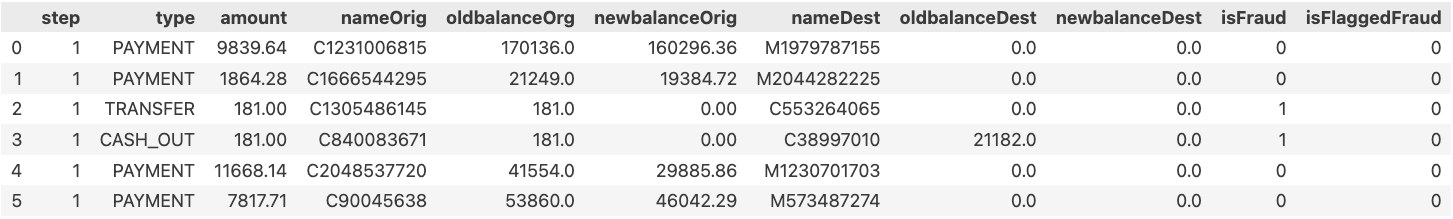
\includegraphics[width=\linewidth]{body/02_methodology/img/figure1.png}
  \caption{Fist 06 rows of the dataset}
\end{figure}

Data we have include both numerical and categorical data, and some of them are not useful for our analysis. Therefore, we need to do some data cleaning and feature engineering to make the data more suitable for our analysis.